
%%%%%%%%%%%%%%%%%%%%%%%%%%%%%%%%%%%%%%%%%%%%%%%%%%%%%%%%%%%%%%%%%%%%%%%%%%%%%
%% Descr:       Vorlage für Berichte der DHBW-Karlsruhe, Ein Kapitel
%% Author:      Prof. Dr. Jürgen Vollmer, vollmer@dhbw-karlsruhe.de
%% $Id: kapitel2.tex,v 1.5 2017/10/06 14:02:51 vollmer Exp $
%%  -*- coding: utf-8 -*-
%%%%%%%%%%%%%%%%%%%%%%%%%%%%%%%%%%%%%%%%%%%%%%%%%%%%%%%%%%%%%%%%%%%%%%%%%%%%%%%

\chapter{Umsetzung}
\label{chap:Umsetzung}
Dieses Kapitel greift die in der Konzeption (\ref{chap:Konzeption}) aufgeführten Planungen und Ideen auf und legt die Implementierung, bzw. 
Umsetzung detaillierte dar. Darunter werden Lösungsansätze aufgezeigt und aufgetretene Probleme und deren Behebung dokumentiert. Allgemein die Umsetzung 
des Startmenüs und der beiden Kernfunktionen sowohl die Frontend- als auch die Backend-Aspekte werden in der Implementierung (\ref{chap:implementierung}) 
aufgezeigt. Abschließend zu dem Kapitel wird ein Szenario dargestellt, indem die Anwendung beschrieben wird.

\section{Implementierung}
\label{chap:implementierung}
Nachdem die Konzeption endgültig abgeschlossen war, ging es an die Umsetzung des Konzepts und an die Implementierung der Funktionen, die das System 
ausmachen. 
\\ 
Die Use Cases und deren Implementierung wurden nach logischer und chronologischer Reihenfolge entwickelt und dokumentiert. Diese festgelegte Reihenfolge 
ist auch der Abbildung (\ref{pic:anwendungsfall}) zu entnehmen. Angefangen mit dem Startmenü, das dem Nutzer die Möglichkeit offenbart zwischen den Funktion 
zu wählen, folgt die Implementierung der Scan-Phase, in der die realen Objekte virtualisiert und platziert werden. Zu guter Letzt die Visualisierungs-Phase, 
welche aufbauend auf die Scan-Phase funktioniert und die zuvor gescannten Objekte erneut virtuell platziert. 
\\ 
Bei erstem Gebrauch der Anwendung ist eine vorzeitige Nutzung der Visualisierungs-Phase ohne weiteres nicht möglich, da zuvor ein Scan durchgeführt 
werden muss, der Daten generiert, Informationen liefert und diese zur Verfügung stellt. Sodass die zweite Kernfunktion operieren kann.
\\ 
\linebreak 
Aufgeteilt wurden die Use Cases der Anwendung jeweils immer nach Frontend und Backend, demnach wird auch die Dokumentation in diesem Stil geschildert. 
\\ 
\linebreak
Bevor die Umsetzung durchgeführt werden konnte, wurden vorab noch die letzten Vorbereitungen durchgeführt.
Zum Start der eigentlichen Implementierung war es die Aufgabe, die Entwicklungsumgebung zu wählen und einzurichten, um bestmöglich arbeiten zu können. Als 
\ac{IDE} wurde die speziell für Android-Applikationen entwickelte Software \textit{Android Studio} gewählt. Diese ist besonders für die Entwicklung von 
Android-Applikation geeignet, ausschließlich für Hardware dessen Software das Android Betriebssystem nutzt. 
\\
Android Studio ist von Google LLC. und JetBrains entwickelt und basiert auf der IntelliJ IDEA Community Edition \acs{IDE}. Als 
Build-Management-Automatisierungs-Tool stellt Android Studio das Tool Gradle zur Verfügung, welches die zu bauenden Projekte durch die verwendeten 
Dependencies, Frameworks und Tools beschreibt. Hier werden unter 
anderem die Bibliotheken und deren verwendete Version eingetragen, um die notwendigen Libraries in der Applikation verwenden zu können. Im Fall des zu 
entwickelnden Unterstützungssystems wurden dort die Bibliotheken zur Nutzung der Android Architecture Components eingetragen, darunter Room und LiveData. 
Darüber hinaus wird dort auch die Version des ARCore Frameworks und des Sceneform \acs{SDK}s verwaltet, welches ebenso essentielle Bestandteile der 
Applikation sind.
\\ 
Nachdem alle Abhängigkeiten erfolgreich eingebunden waren, wurden zur übersichtlichen Gestaltung der Klassen, Objekte, ViewModel, Repositories und Activities 
eine Ordnerstruktur angelegt, die alle Klassen des gleichen Typs im Laufe der Entwicklung beinhalten sollen. Dadurch kann besser und übersichtlicher durch 
das Projekt navigiert werden und alle Klassen ähnlicher Eigenschaften befinden sich im selben Zielordner. Nachdem nun alle Vorbereitungen abgeschlossen 
waren, ging es an die Entwicklung des ersten Use Cases, dem Startmenü, um die Grundlage des Systems zu festigen.  

\subsection{Startmenü}
Das Startmenü ist die zentrale Anlaufstelle des prototypischen Unterstützungssystems und bildet den Einstiegspunkt in die Interaktionen mit der Applikation.
\\ 
Nun folgt die Beschreibung der Implementierung des Startmenüs, sowohl des Frontends als auch des Backends.

\subsubsection{FrontEnd}
Wird das Unterstützungssystem heruntergeladen oder auf die verwendete Hardware geladen, folgt das Speichern der Anwendung auf dem Gerät. Die Applikation erscheint 
auf dem Applikationshauptmenü des Smart-Devices und wird dort zur Nutzung zur Verfügung gestellt. 
\begin{figure}[hbt!]
    \centering
    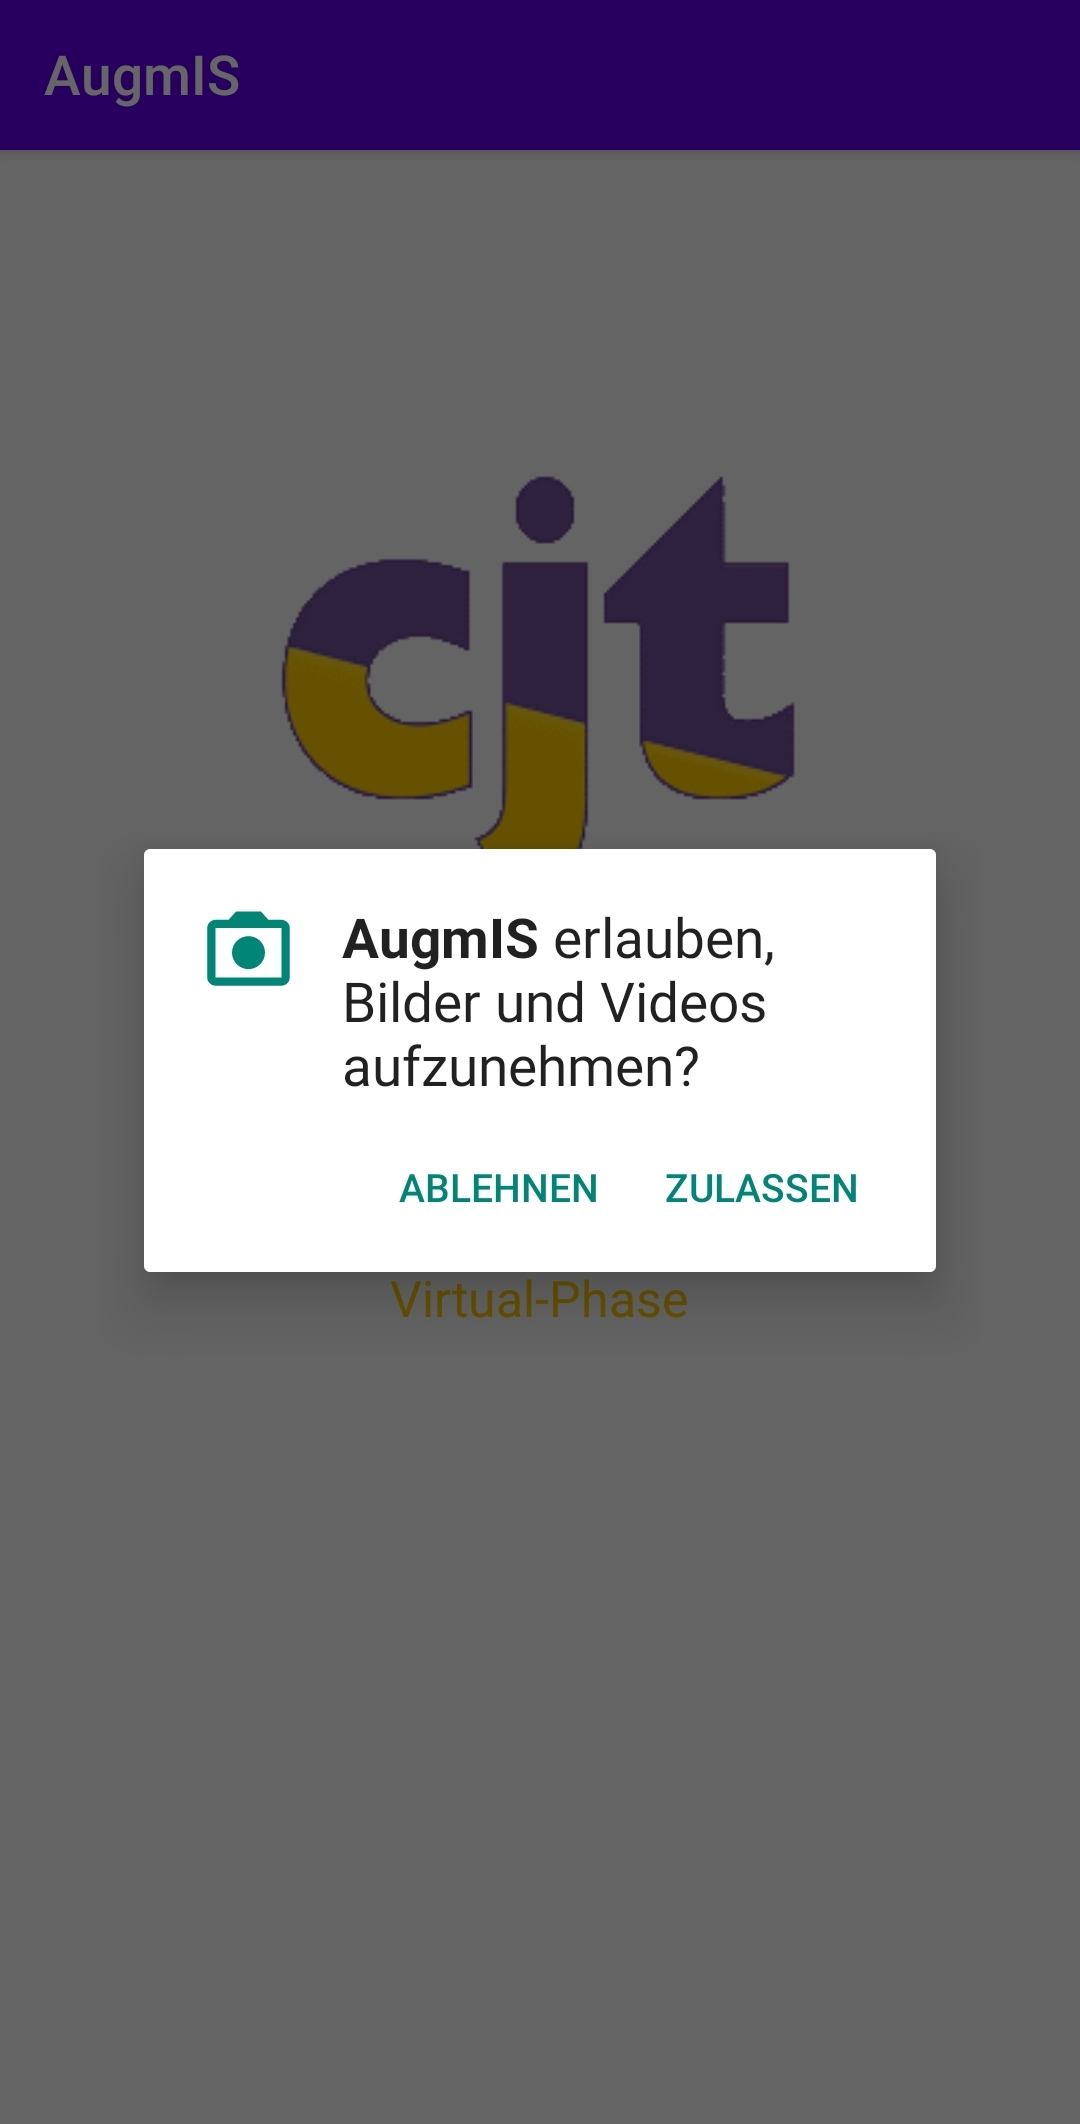
\includegraphics[width=10cm,height=7.5cm,keepaspectratio]{4Umsetzung/Bilder/camera_permission.jpg}
    \caption{Start der Applikation}
    \label{pic:camera_perm}
\end{figure}
\begin{figure}[hbt!]
    \centering
    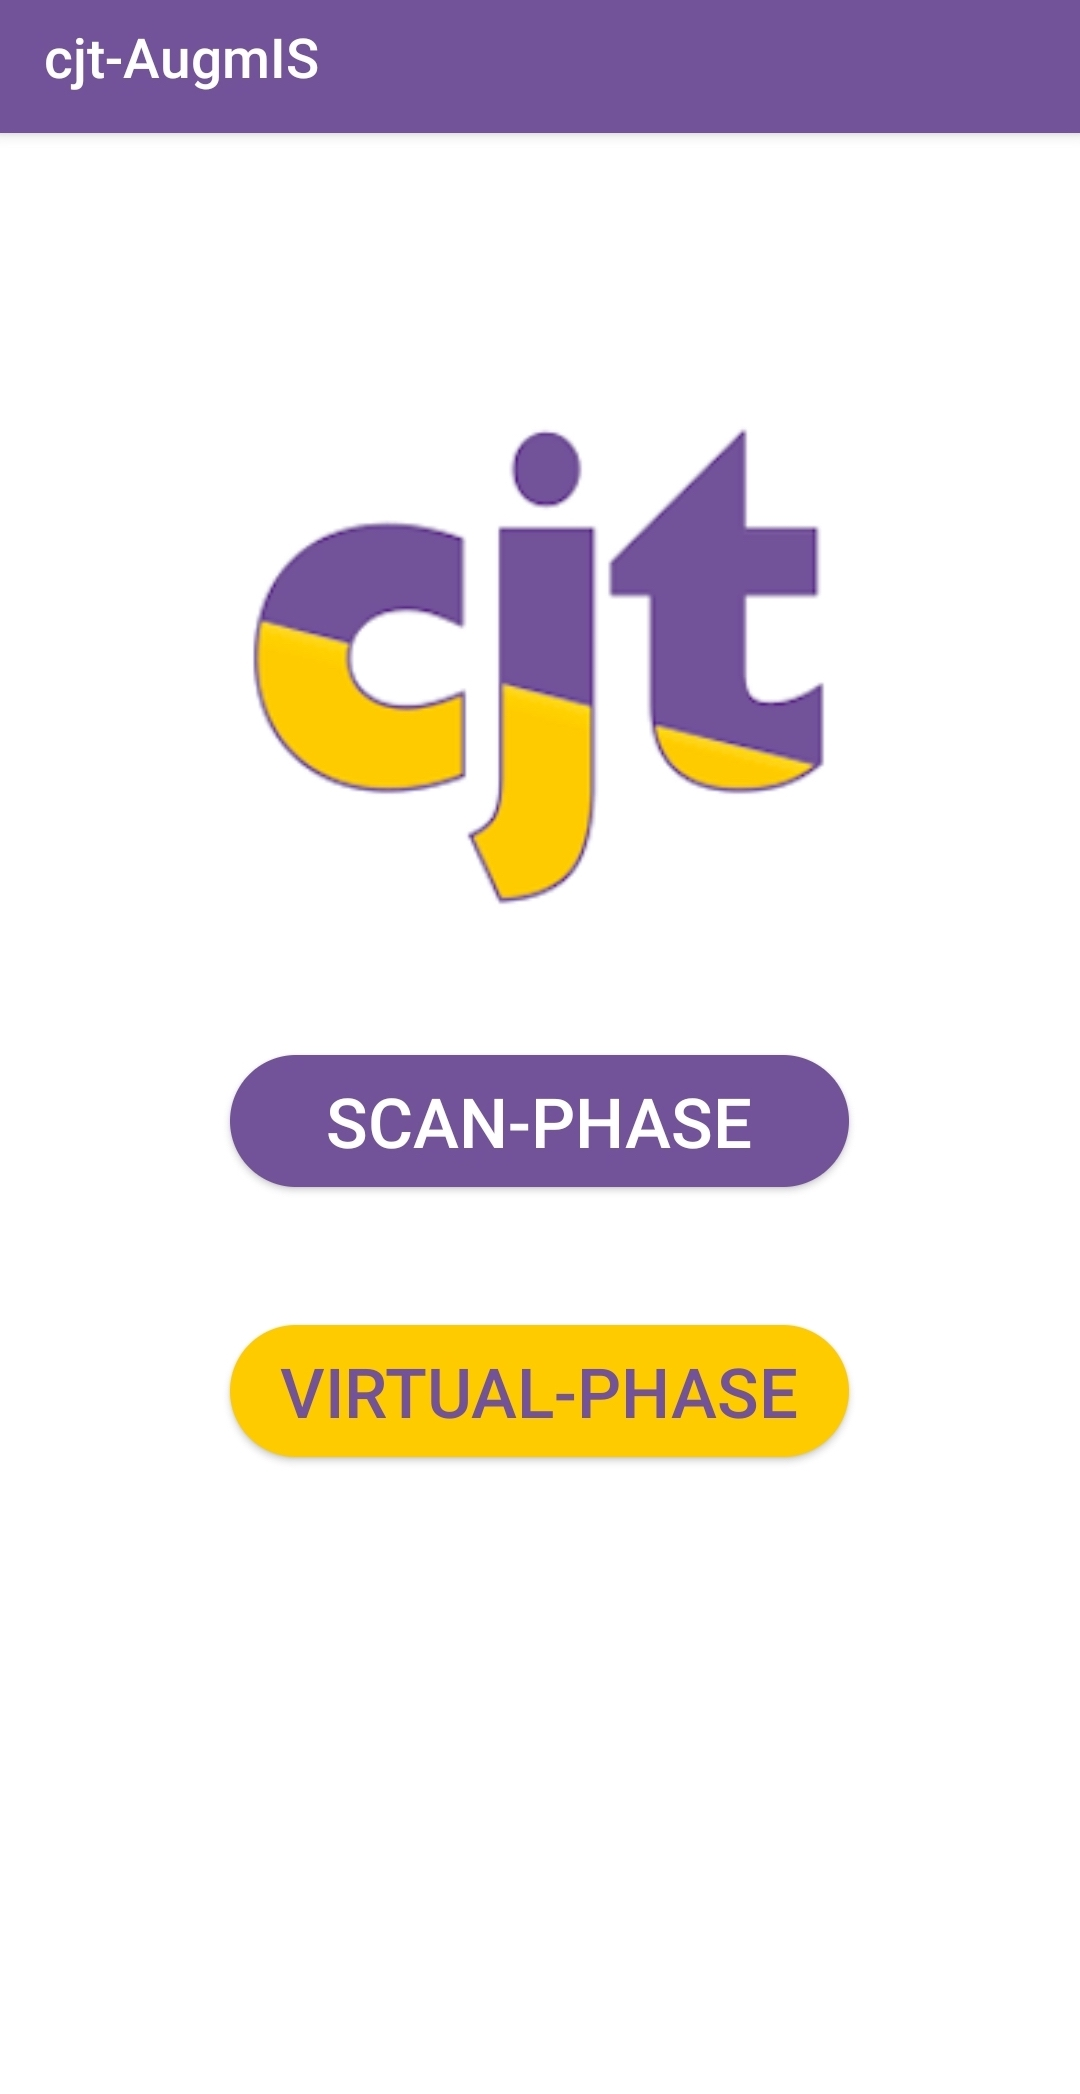
\includegraphics[width=10cm,height=7.5cm,keepaspectratio]{4Umsetzung/Bilder/startmenu.jpg}
    \caption{Startmenü der Applikation}
    \label{pic:startmenu}
\end{figure}
\subsubsection{BackEnd}

\subsection{Scan-Phase} %Umgebungserkennung /
\subsubsection{FrontEnd}
\begin{figure}[hbt!]
    \centering
    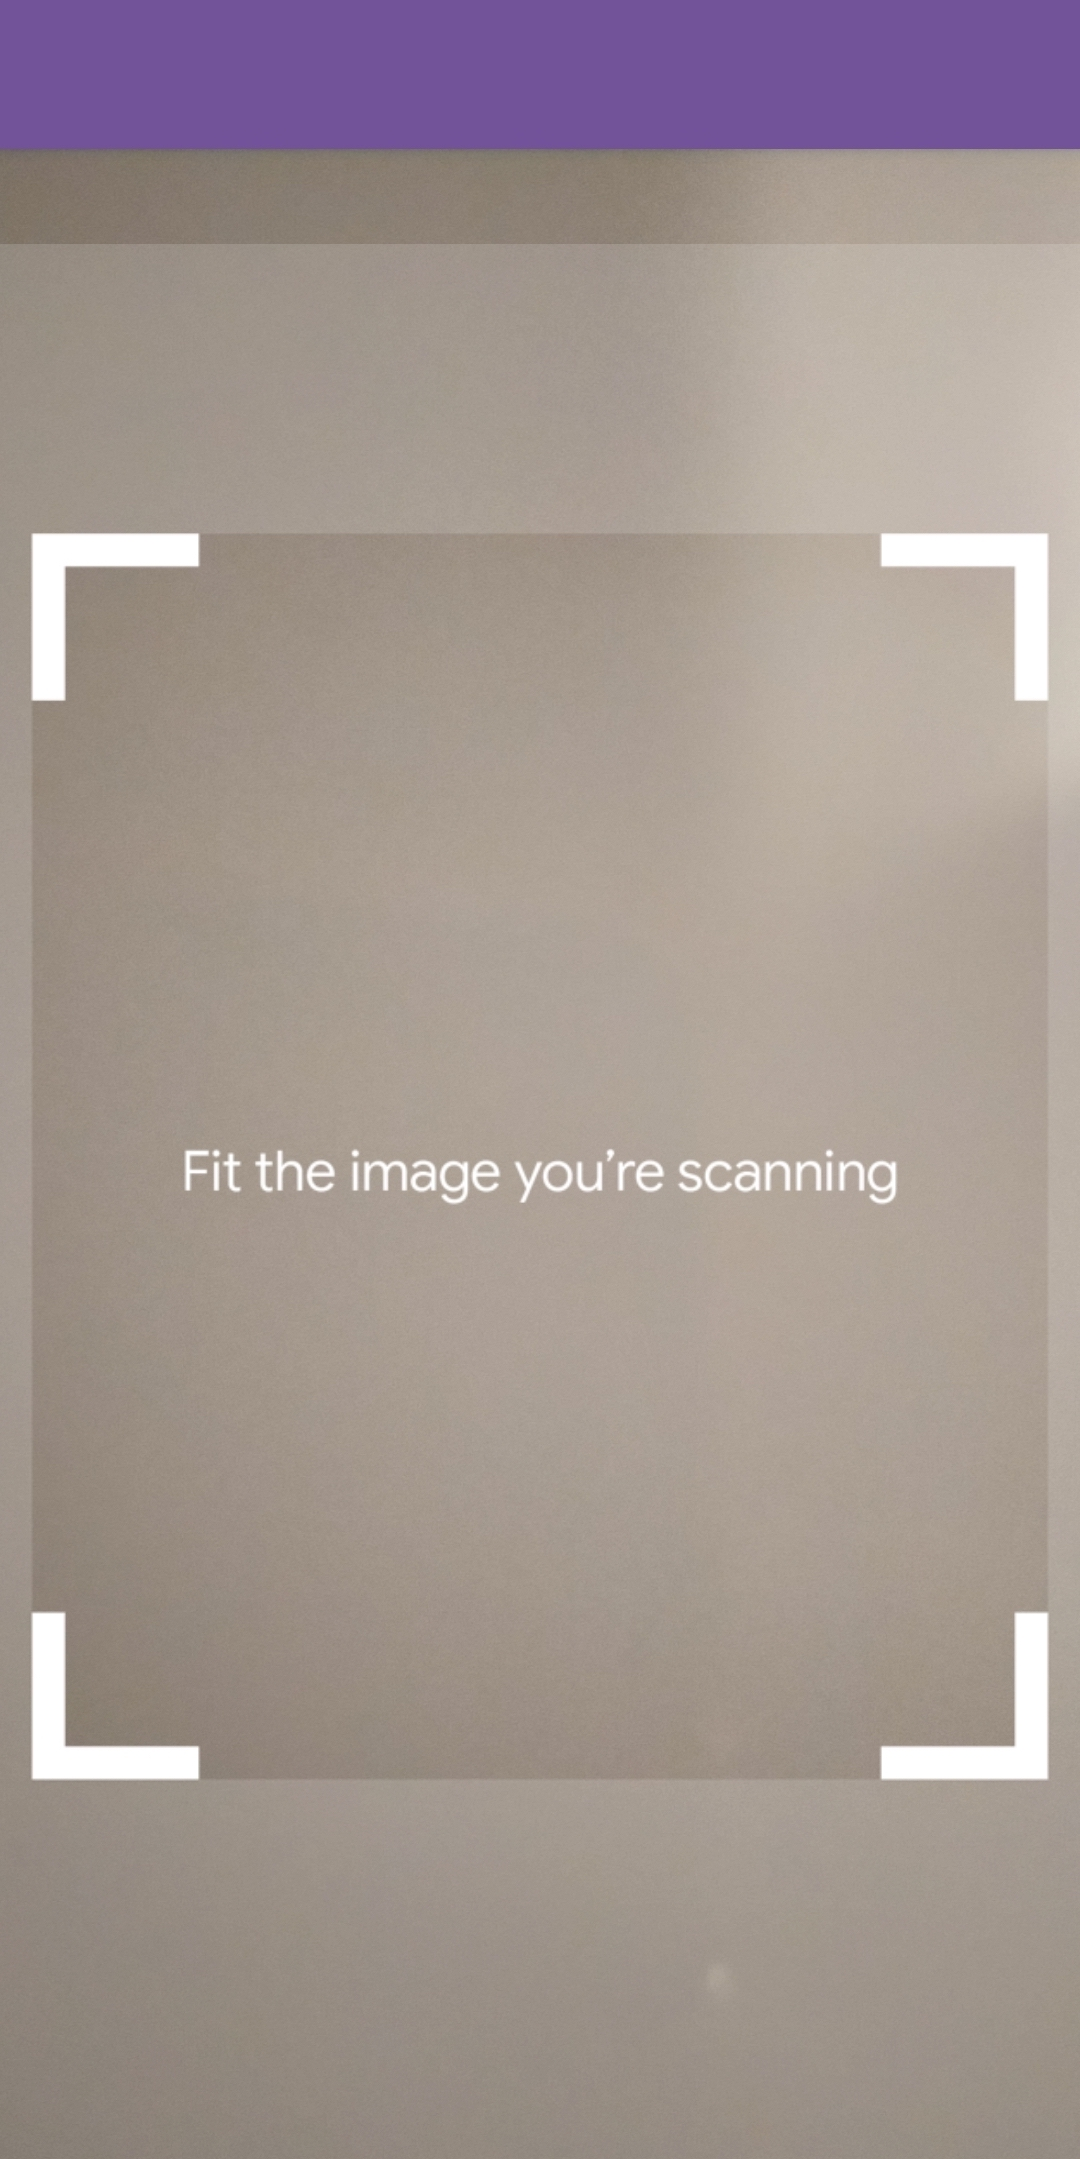
\includegraphics[width=10cm,height=7.5cm,keepaspectratio]{4Umsetzung/Bilder/image_tracking.jpg}
    \caption{Markererkennung der Applikation zum Start der Scan-Phase}
    \label{pic:image_tracking}
\end{figure}
\begin{figure}[hbt!]
    \centering
    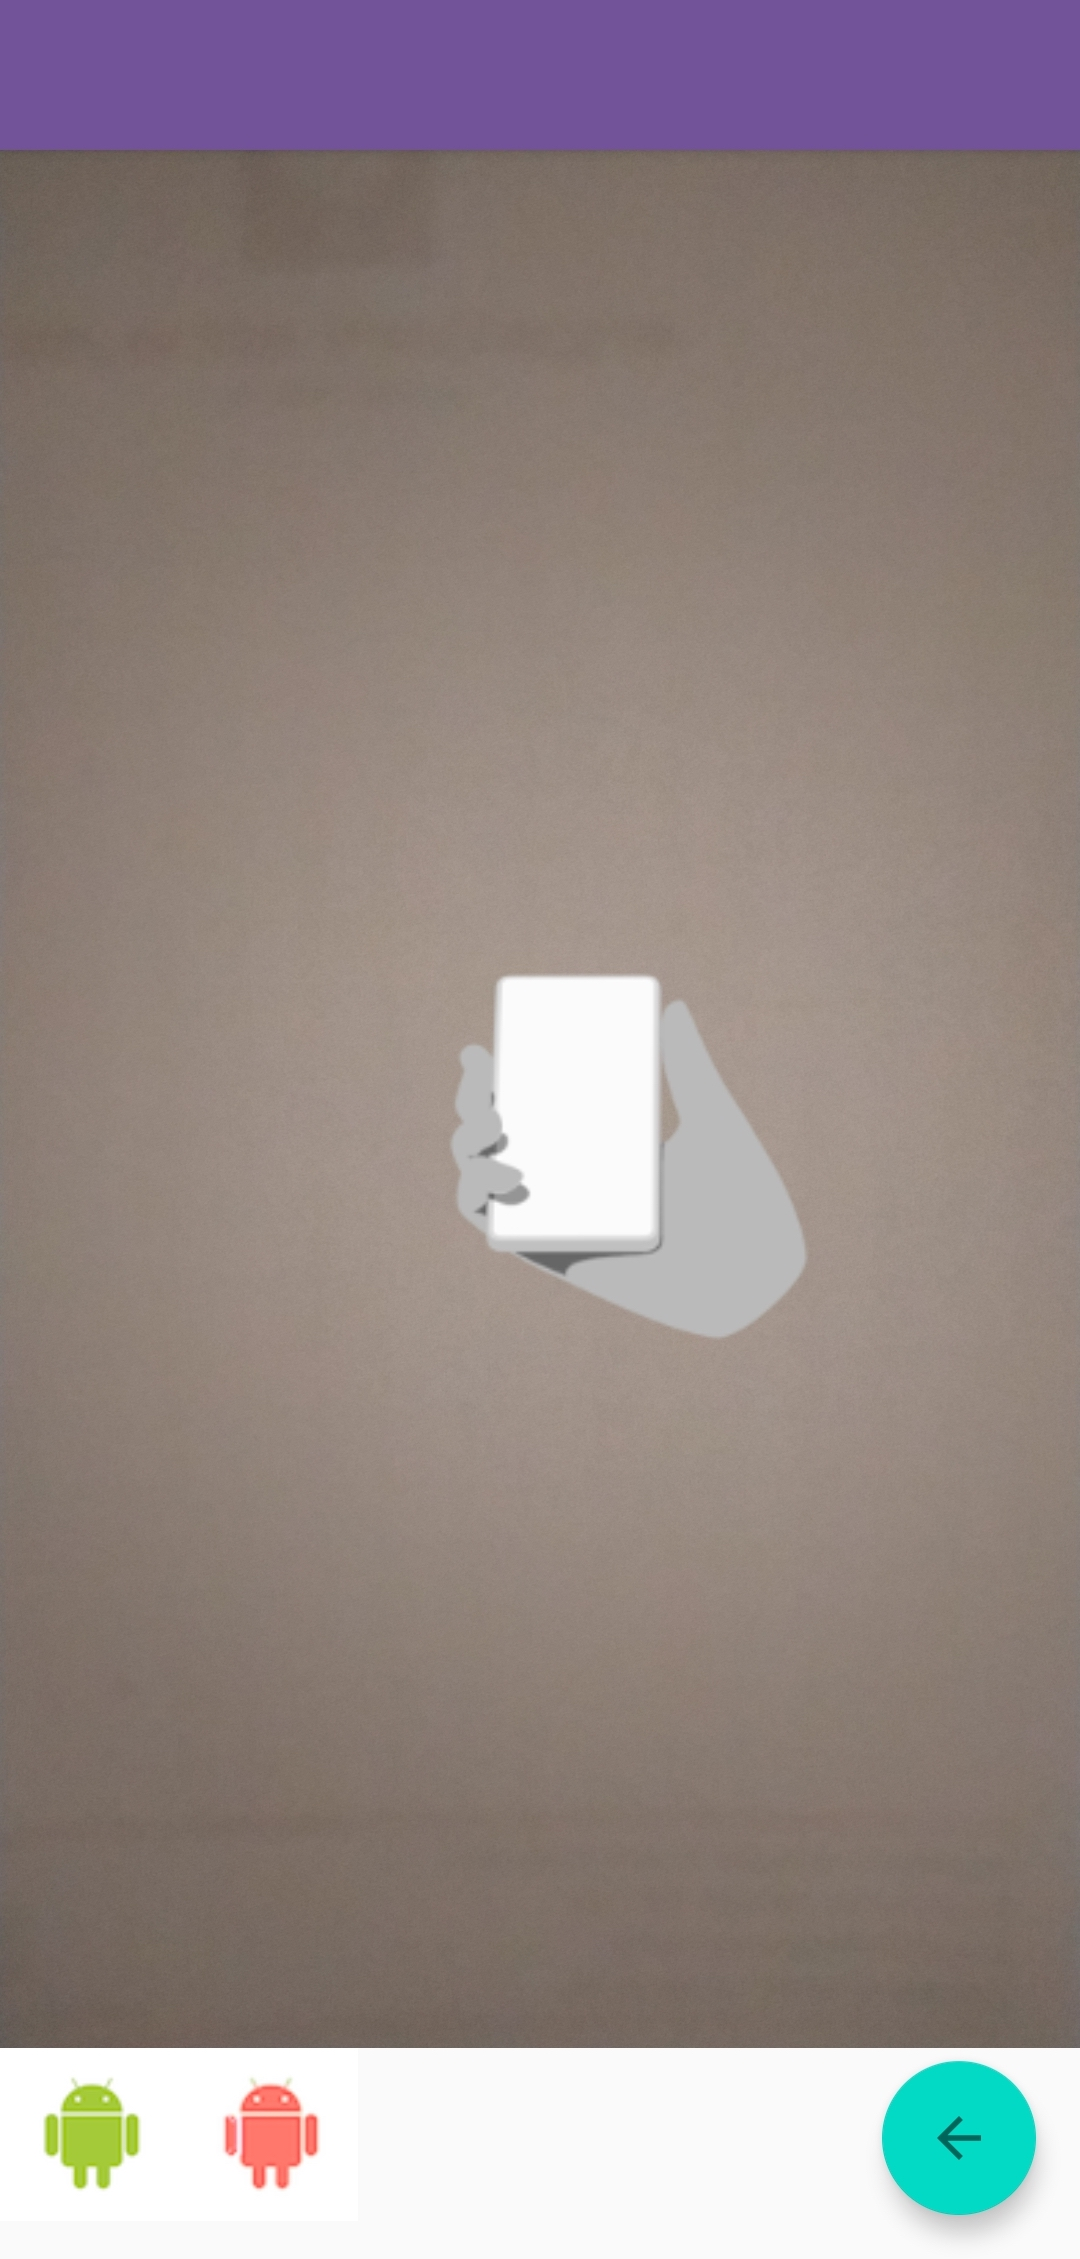
\includegraphics[width=10cm,height=7.5cm,keepaspectratio]{4Umsetzung/Bilder/scan-phase.jpg}
    \caption{Scan-Phase der Applikation}
    \label{pic:scan}
\end{figure}
\subsubsection{BackEnd}
\begin{figure}[hbt!]
    \centering
    
\includegraphics[width=5cm,height=5cm,keepaspectratio]{4Umsetzung/Bilder/cjt_logo_tracking.png}
    \caption{Marker zur Erkennung der Ausgangsposition}
    \label{pic:initialMarker}
\end{figure}

\subsection{Visualisierungs-Phase} 
\subsubsection{FrontEnd}
\begin{figure}[hbt!]
    \centering
    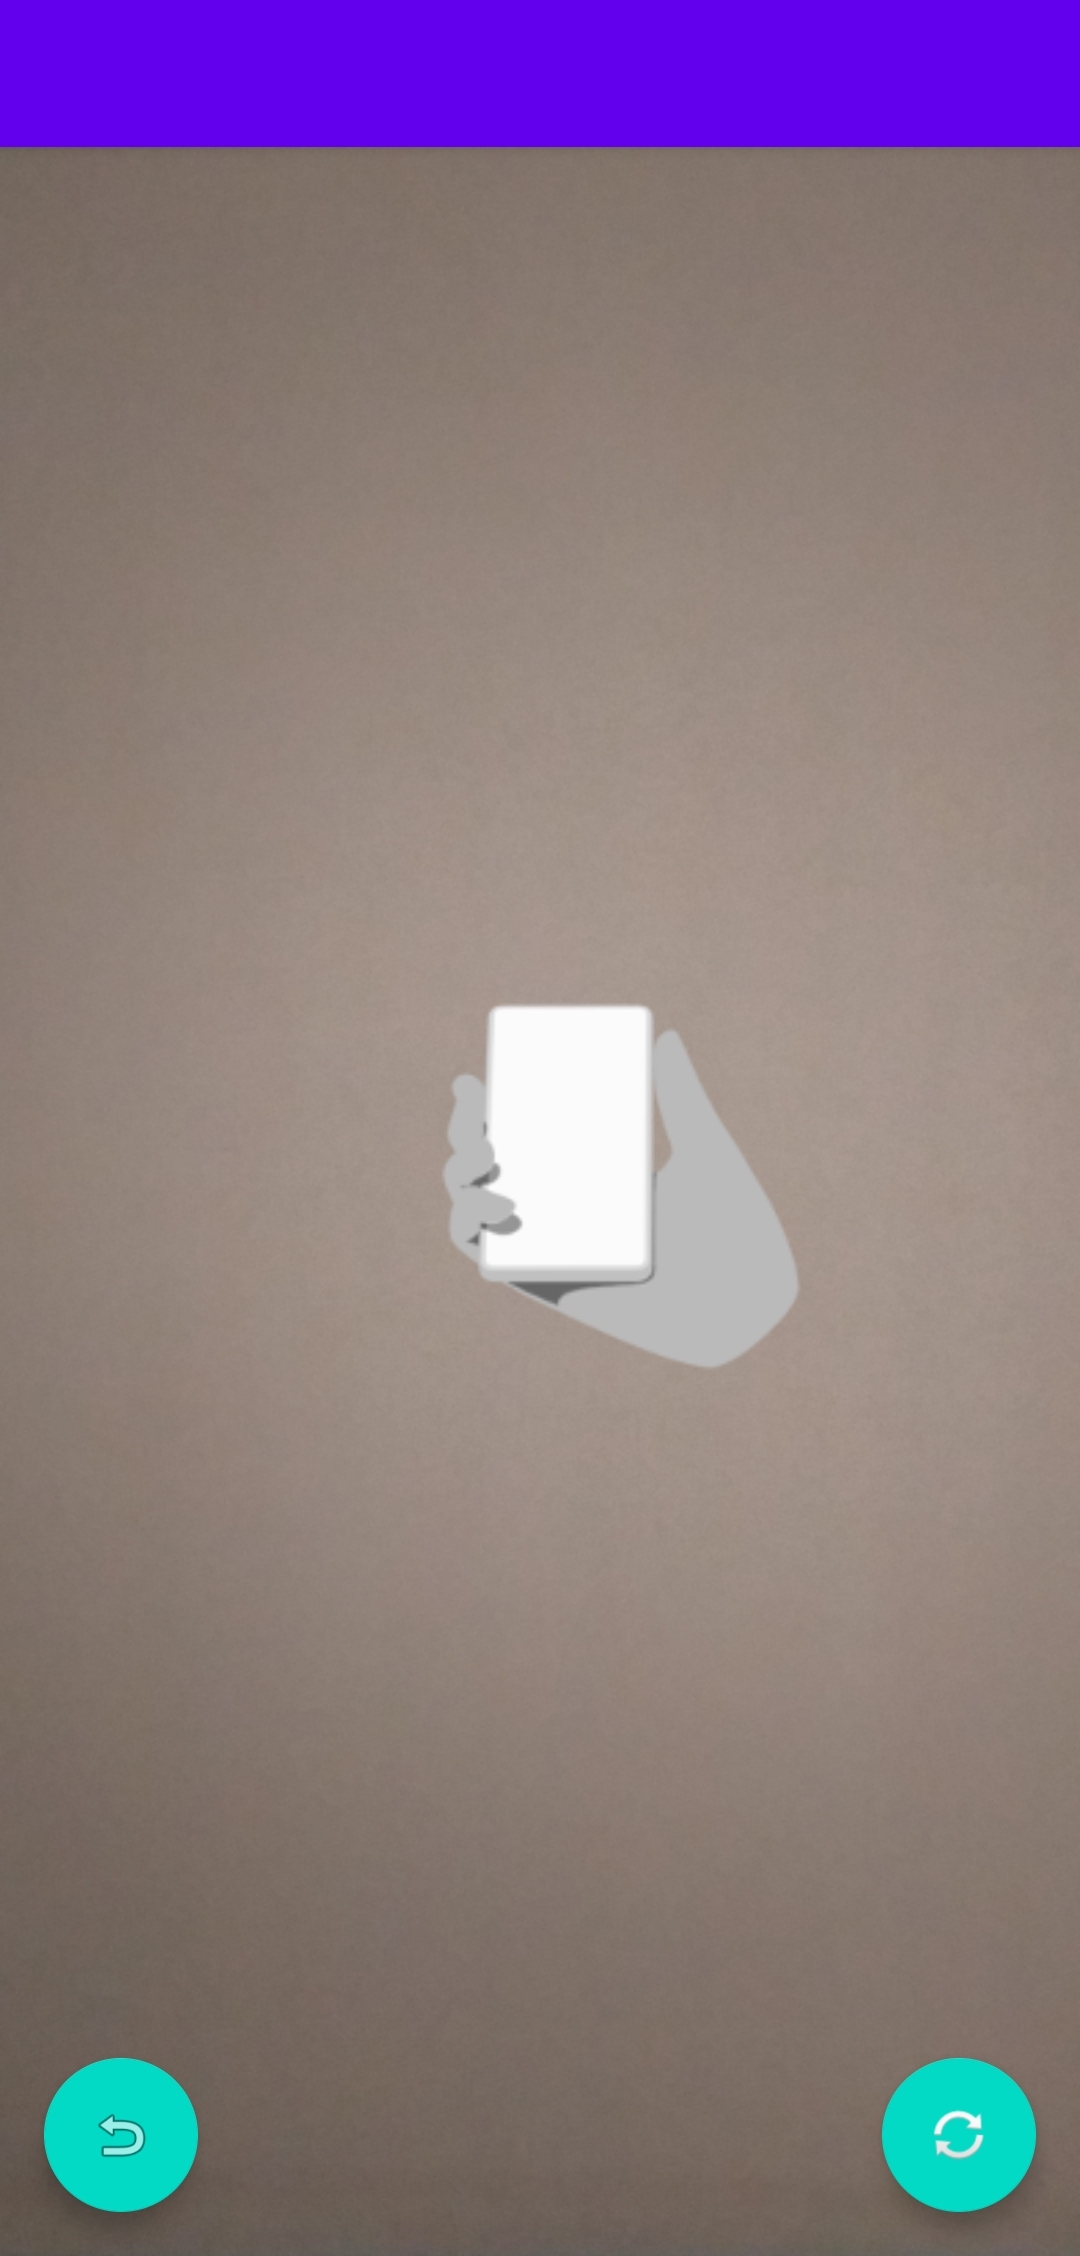
\includegraphics[width=10cm,height=7.5cm,keepaspectratio]{4Umsetzung/Bilder/visual-phase.jpg}
    \caption{Visualisierungs-Phase der Applikation}
    \label{pic:visual}
\end{figure}
\subsubsection{BackEnd}

\section{Testdurchlauf / Test-Szenario}
\label{chap:testdurchlauf}